\documentclass[a4paper,14pt]{article}
\usepackage{filecontents}

\usepackage[utf8]{inputenc}
\usepackage[english]{babel}
\usepackage{graphicx, array, blindtext}
\usepackage[colorinlistoftodos]{todonotes}
\DeclareUnicodeCharacter{2212}{-}
\usepackage [a4 paper , hmargin = 1.2 in , bottom = 1.5 in] {geometry}
\usepackage [parfill] {parskip}

\usepackage{enumitem}
\usepackage{amsmath}
\usepackage{amsthm}

\usepackage{nameref}
\usepackage{amssymb}
\usepackage [linesnumbered, ruled, vlined] {algorithm2e}
\usepackage{listings}
\usepackage{xcolor}
\usepackage{floatrow}
\usepackage{siunitx}
\usepackage{cancel}
\usepackage{fancyhdr}
\usepackage{graphicx}
\usepackage{verbatim}
\usepackage[document]{ragged2e}

\renewcommand{\footrulewidth}{0.4pt}
\newtheorem{definition}{Definition}
\numberwithin{definition}{section}
\newtheorem{mytheorem}{Theorem}
\numberwithin{mytheorem}{subsection}
\newcommand{\notimplies}{\;\not\!\!\!\longrightarrow}  
\newcommand\norm[1]{\left\lVert#1\right\rVert}
\pagestyle{fancy}
\fancyhf{}
\rhead{CS754 Assignment 5}
\lhead{200050013-200050130}
\fancyfoot[C]{Page \thepage}
\usepackage{subcaption}
\usepackage{listings}


\usepackage{hyperref}
\urlstyle{same}
\hypersetup{pdftitle={main.pdf},
    colorlinks=false,
    linkbordercolor=red
}
\usepackage{array}
\usepackage{listings,chngcntr}

\begin{document}
\centering{

\title{\fontsize{150}{60}{CS754 Assignment 5 Report}}

\author{
Arpon Basu \\ Shashwat Garg }
}

\date{Spring 2022}
\maketitle

\justifying
\tableofcontents

\newpage
\justifying
\section*{Introduction}

Welcome  to our report on CS754 Assignment 5. We have tried to make this report comprehensive and self-contained. We hope reading this would give you a proper flowing description of our work, methods used and the results obtained.

Also note that we installed the \texttt{Image Processing Toolbox} in MATLAB for this assignment. Thus the grader is urged to install it if she wishes to run the code on her on her machine. Also note that some of our code may take a while to run because of the intensive nature of the computations involved.

Hope you enjoy reading the report. Here we go!
\section{Problem 1}
\subsection{(a)}
\subsection{(b)}
The likelihood was Laplacian.\\
The terms involving the likelihood were 
$$\sum_{i, k}\rho(f_{i,k}\cdot I_1)\;\mathrm{and}\;\rho(f_{i,k}\cdot (I-I_1))$$
The log-histogram of derivative filters was the prior.
The terms involving the prior were 
$$\sum_{i, k}\rho(f_{i,k}\cdot I_1)\;\mathrm{and}\;\rho(f_{i,k}\cdot (I-I_1))$$
\subsection{(c)}
Note that since we have to remove reflections from natural images, we have to somehow distinguish between natural images and artificial reflections. That is done by exploiting the property of natural images that the log-histograms of the derivatives of the image (obtained through some derivative filter) are sparse, and thus they decay rapidly away from zero (of the x-axis), thus giving them a \textbf{convex nature}.\\
Thus, \textbf{Gaussian likelihoods aren't chosen because they are concave in nature}, ie:- they decay more slowly than one would expect from a natural image. On the other hand, for a Laplacian likelihood, the log histogram is straight decreasing line, which basically delineates the boundary between sparse and non-sparse likelihoods. In general, one may say that likelihoods of the form $e^{-x^\alpha}$ are better than likelihoods of the form $e^{-x^\beta}$ if $\alpha < \beta$, and thus since $1 < 2$, a Laplacian is a better likelihood than the Gaussian.
\begin{figure}[H]
    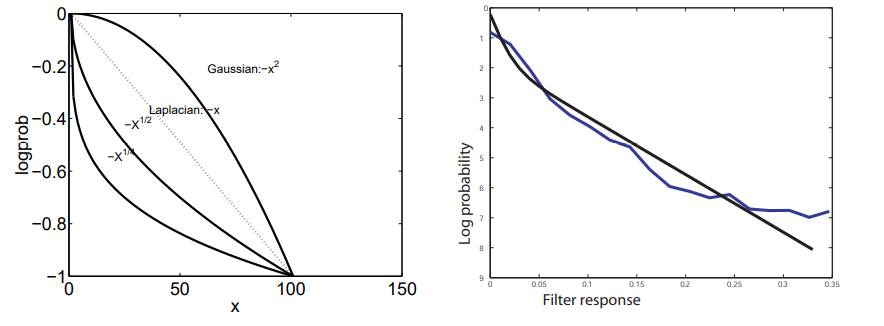
\includegraphics{Q1.png}
    \caption{Graph highlighting better sparsity of Laplacian vis-a-vis Gaussian}
\end{figure}
\section{Problem 2}
From the machinery of Baye's theorem we know that the \textbf{Maximum A Posteriori Estimate} $\boldsymbol{x}$ is given by
$$\boldsymbol{x} = \mathrm{arg\;max}_x p(x|y)$$
But we also know that
$$p(x|y)\propto p(x)p(y|x)$$
Now, since $x\sim\mathcal{N}(0,\Sigma_x)$, we have that (we ignore differentials and just quote the value of the PDF of the multivariate Gaussian)
$$p(x) = \frac{1}{\sqrt{(2\pi)^n|\Sigma_x|}}\mathrm{exp}(-\frac{1}{2}x^T\Sigma_x^{-1}x)$$
Also, note that that $p(y|x)$ denotes how likely $y$ is to be obtained if $x$ is the input vector from which it was created. But note that this is equivalent to asking how likely is $\eta = y - \Phi x$ to have come from the given noise distribution $\mathcal{N}(0, \sigma^2I_{m\times m})$. Thus
$$p(y|x) = p(\eta) = \frac{1}{\sqrt{(2\pi)^m\sigma^{2m}}}\mathrm{exp}(-\frac{1}{2\sigma^2}\lVert\eta\rVert^2_2) = \frac{1}{\sqrt{(2\pi)^m}\sigma^{m}}\mathrm{exp}(-\frac{1}{2\sigma^2}\lVert y-\Phi x\rVert^2_2)$$
where we plugin the scalar (a multiple of the identity matrix) covariance matrix to derive the neat form seen above.
Thus, when we plugin the expressions (and remove all the constants), we get
$$p(x|y) \propto \mathrm{exp}(-\frac{1}{2}(\frac{1}{\sigma^2}\lVert y-\Phi x\rVert^2_2 + x^T\Sigma_x^{-1}x))$$
Thus maximizing $p(x|y)$ is equivalent to minimizing $(\frac{1}{\sigma^2}\lVert y-\Phi x\rVert^2_2 + x^T\Sigma_x^{-1}x)$ given $y$ and $\Phi$.\\
Differentiating the expression w.r.t the vector $\boldsymbol{x}$, we get
$$\frac{\partial(\frac{1}{\sigma^2}\lVert y-\Phi x\rVert^2_2 + x^T\Sigma_x^{-1}x)}{\partial x} = 0$$
$$\implies \frac{1}{\sigma^2}(2\Phi^T\Phi x - 2\Phi^Ty) + 2\Sigma_x^{-1}x = 0$$
$$\implies (\Phi^T\Phi + \sigma^2\Sigma_x^{-1})x = \Phi^Ty$$
$$\implies \boldsymbol{x}_{\mathrm{MAP}} = (\Phi^T\Phi + \sigma^2\Sigma_x^{-1})^{-1}\Phi^Ty$$
\begin{figure}
    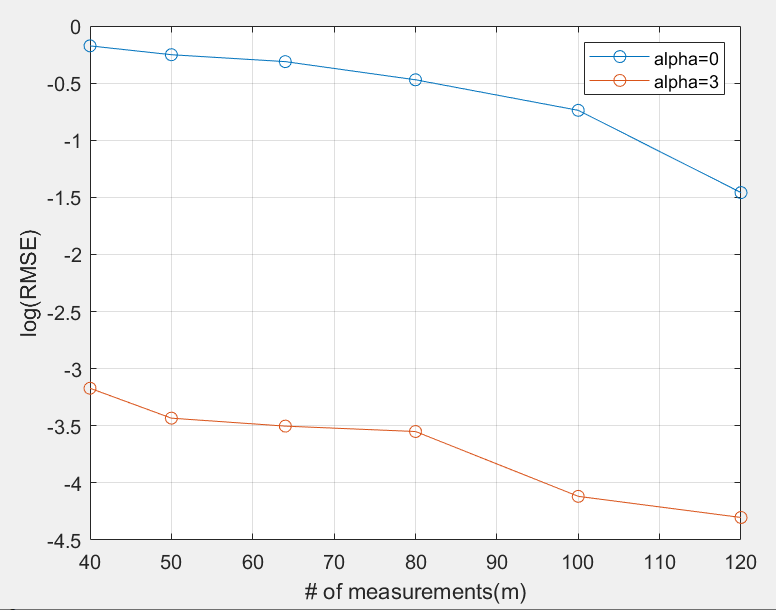
\includegraphics{Q2.png}
    \caption{Errors obtained for various $m$'s for $\alpha = 0$ and $\alpha = 3$}
\end{figure}
Note that the errors here have been plotted on log-scale to better highlight the differences between them. As one can see, there is indeed a noticeable difference in the reconstruction accuracy for $\alpha = 0$ and $\alpha = 3$. We would like to explain this phenomena as a combination of two observations:
\begin{itemize}
    \item RMSE decreases as $m$ increases for a given $\alpha$: This is quite intuitive since more samples of $\boldsymbol{x}$ will obviously increase the accuracy of our Bayesian estimate.
    \item RMSE decreases as $\alpha$ increases for a given $m$: Note that for higher $\alpha$, the eigenvalues of our covariance matrix $\Sigma_x$ fall of very rapidly, and thus, a random variable $\boldsymbol{x}$ sampled from a probability distribution with $\Sigma_x$ as the covariance matrix will vary very little in the directions of the principal eigenvectors of those small eigenvalues, thus essentially ``reducing" the ``effective" dimension of the vector $\boldsymbol{x}$ (one may note that this is the very insight of PCA, which recognizes that one may effectively set the very small eigenvalues to 0). Thus, for larger $\alpha$, we effectively have to interpolate ``smaller" $\boldsymbol{x}$, and hence the better reconstruction accuracy.
\end{itemize}
\section{Problem 3}
In this problem we'll deal with the problem below.\\
Let $X^*$ be the solution of the optimization problem given below
$$X^* := \arg \min \limits_{X} \norm{X}_* \quad \text{subject to } \mathcal{A}(X) = b$$
and let $X_0$ be \emph{any} matrix of rank $r$ such that $\mathcal{A}(X_0) = b$. We will be investigating under what conditions will $X^*$ necessarily equal $X_0$.
\subsection{3(a)}
$X^*$ is the matrix of minimum $\lVert\cdot\rVert_*$ norm subject to the constraint $\mathcal{A}(X) = b$. Now, $X_0$ belongs to our search space since by the hypothesis of the theorem $\mathcal{A}(X_0) = b$. And since we optimize the $\lVert\cdot\rVert_*$ norm over our search space to get $X^*$, we have that
$$\lVert X^*\rVert_* \leq \lVert X_0\rVert_*$$
\subsection{3(b)}
By the very definition of $R_c$, as also written two lines above where this question was posed, we have that $X_0^{\prime}R_c$ and $X_0R_c^{\prime}$ are both zero (matrices). Thus, applying Lemma 2.3 verbatim (which states that if two matrices $A$ and $B$ of equal dimensions satisfy $A^{\prime}B = 0$ and $AB^{\prime} = 0$, then $\lVert A+B\rVert_* = \lVert A\rVert_* + \lVert B\rVert_*$), we get that $\lVert X_0+R_c\rVert_* = \lVert X_0\rVert_* + \lVert R_c\rVert_*$, since $X_0$ and $R_c$ are clearly of equal dimensions ($R = X^* - X_0$, $R = R_0 + R_c$, thus implying that $X_0$ and $R_c$ are addable, and thus of equal dimensions) and satisfy $X_0^{\prime}R_c = 0$ and $X_0R_c^{\prime} = 0$.
\subsection{3(c)}
WLOG assume that the singular values of $R_c$ are arranged in descending order, ie:- $\sigma_i \leq \sigma_j$ for any $i\geq j$. Then note that if $k\in I_{i+1}$, then $\sigma_k\leq\sigma_j$ $\forall j\in I_i$ since $k$ is a larger index. Thus
$$3r\cdot\sigma_k\leq\sum_{j\in I_i}\sigma_j\;\forall\;k\in I_{i+1}$$
by adding up all the inequalities individually, and thus, finally
$$\sigma_k\leq\frac{1}{3r}\sum_{j\in I_i}\sigma_j\;\forall\;k\in I_{i+1}$$
\subsection{3(d)}
For this problem, we recall a linear algebra property which says that for any matrix $M$, we have that
$$\lVert M\rVert_F^2 = \sum^{n}_{i = 1}\sigma^2_i$$
where $\sigma_1$, $\sigma_2$, ..., $\sigma_n$ are the singular values of $M$. One can easily see this by observing that $\lVert M\rVert_F^2 = \mathrm{tr}(MM^\prime)$. But the trace of a matrix is equal to the sum of it's eigenvalues, and the eigenvalues of $MM^\prime$ are the squares of the singular values of $M$.\\
Also note that the $\lVert\cdot\rVert_*$ norm is defined as
$$\lVert X\rVert_* = \sum_{\sigma\mathrm{\;is\;a\;singular\;value\;of\;X}} \sigma$$
Thus
$$\sigma_k\leq\frac{1}{3r}\sum_{j\in I_i}\sigma_j = \frac{1}{3r}\lVert R_i\rVert_*\;\forall\;k\in I_{i+1}$$
$$\implies \sigma^2_k\leq\frac{1}{9r^2}\lVert R_i\rVert_*^2\;\forall\;k\in I_{i+1}$$
$$\implies\sum_{k\in I_{i+1}}\sigma^2_k \leq 3r\frac{1}{9r^2}\lVert R_i\rVert_*^2$$
But then we also know that
$$\lVert R_{i+1}\rVert^2_F = \sum_{k\in I_{i+1}}\sigma_j^2$$
Thus
$$\lVert R_{i+1}\rVert^2_F \leq \frac{1}{3r}\lVert R_i\rVert_*^2$$
as desired.
% $$\lVert R_{i+1}\rVert^2_F = \sum_{j\in I_{i+1}}\sigma_j^2\leq\sum_{j\in I_{i+1}}\frac{1}{9r^2}(\sum_{l\in I_{i}}\sigma_l)^2$$
% Now applying the RMS-AM inequality we get
% $$(\sum_{l\in I_{i}}\sigma_l)^2 \leq |I_{i}|\sum_{l\in I_{i}}\sigma_l^2 = 3r\sum_{l\in I_{i}}\sigma_l^2$$
% Tying everything up, 
% $$\lVert R_{i+1}\rVert^2_F = \sum_{j\in I_{i+1}}\sigma_j^2\leq\sum_{j\in I_{i+1}}\frac{1}{9r^2}(\sum_{l\in I_{i}}\sigma_l)^2\leq\sum_{j\in I_{i+1}}\frac{1}{9r^2}3r\sum_{l\in I_{i}}\sigma_l^2 = \frac{3r\cdot 3r}{9r^2}\sum_{l\in I_{i}}\sigma_l^2 = \lVert R_{i}\rVert^2_F$$
\subsection{3(e)}
We know from the previous part that
$$\lVert R_{i+1}\rVert^2_F \leq \frac{1}{3r}\lVert R_i\rVert_*^2$$
$$\implies \lVert R_{i+1}\rVert_F \leq \frac{1}{\sqrt{3r}}\lVert R_i\rVert_*$$
$$\implies \sum^{t-1}_{i = 1}\lVert R_{i+1}\rVert_F \leq \sum^{t-1}_{i = 1}\frac{1}{\sqrt{3r}}\lVert R_i\rVert_*\leq \sum^{t}_{i = 1}\frac{1}{\sqrt{3r}}\lVert R_i\rVert_*$$
$$\implies \sum_{i \geq 2}\lVert R_{i}\rVert_F \leq\sum_{i \geq 1}\frac{1}{\sqrt{3r}}\lVert R_i\rVert_*$$
as desired, where there are $t$ matrices $\{R_i\}_{1\leq i\leq t}$.
\subsection{3(f)}
Note that the justification we gave for 3(b) was basically to prove that $\lVert R_0\rVert_* \geq \lVert R_c\rVert_*$. We proceed on that as follows
$$\lVert X_0\rVert_* \geq \lVert X^*\rVert_* = \lVert X_0 + R\rVert_*$$
where $R := X_0 - X^*$. Then
$$\lVert X_0\rVert_* \geq \lVert X_0 + R\rVert_* = \lVert X_0 + R_c + R_0\rVert_* \geq \lVert X_0 + R_c\rVert_* - \lVert R_0\rVert_*$$
where the last inequality follows by the triangle inequality. But in part (b) we just proved that $\lVert X_0 + R_c\rVert_* = \lVert X_0\rVert_* + \lVert R_c\rVert_*$, and thus
$$\lVert X_0\rVert_* \geq \lVert X_0\rVert_* + \lVert R_c\rVert_* - \lVert R_0\rVert_*$$
$$\implies \lVert R_0\rVert_* \geq \lVert R_c\rVert_*$$
as desired.
\subsection{3(g)}
We use a relation from linear algebra which establishes a bound between Frobenius norm and the nuclear norm
$$\boldsymbol{\lVert M\rVert_* \leq \sqrt{\mathrm{rank}\;M}\lVert M\rVert_F}$$
But from it's construction itself (the construction of $R_0$ entails (through Lemma 3.4) that rank$(R_0)\leq 2\cdot$rank$(X_0) = 2r$, since rank$(X_0) = r$) we know that rank$(R_0)\leq 2r$, thus
$$\sum_{i \geq 2}\lVert R_{i}\rVert_F \leq\sum_{i \geq 1}\frac{1}{\sqrt{3r}}\lVert R_i\rVert_* = \frac{1}{\sqrt{3r}}\lVert R_c\rVert_* \leq \frac{1}{\sqrt{3r}}\lVert R_0\rVert_* \leq \frac{\sqrt{\mathrm{rank}\;R_0}}{\sqrt{3r}}\lVert R_0\rVert_F\leq \frac{\sqrt{2r}}{\sqrt{3r}}\lVert R_0\rVert_F$$
as desired.
\subsection{3(h)}
As we have seen above, rank$(R_0)\leq 2r$, and also note that $R_1$ was constructed such that it's rank was atmost 3$r$ (``$R_c = \sum^{t}_{i = 1}R_i$, rank$(R_i)\leq 3r$").\\
Now, we also know that 
$$\mathrm{rank}(A+B)\leq\mathrm{rank}(A) + \mathrm{rank}(B)$$
Thus
$$\mathrm{rank}(R_0 + R_1)\leq\mathrm{rank}(R_0) + \mathrm{rank}(R_1) \leq 2r + 3r = 5r$$
as desired.
\subsection{3(i)}
Note that $\mathcal{A}$ was defined was a linear mapping (from matrices to vectors), and thus
$$\lVert\mathcal{A}(R)\rVert = \lVert\mathcal{A}(R_0 + R_c)\rVert = \lVert\mathcal{A}(R_0 + R_1 + R_2 + \hdots)\rVert = \lVert\mathcal{A}(R_0 + R_1) + \mathcal{A}(R_2 + \hdots)\rVert$$
$$\geq \lVert\mathcal{A}(R_0 + R_1)\rVert - \sum_{j\geq 2}\lVert\mathcal{A}(R_j)\rVert$$
where the last inequality follows by the triangle inequality (note that $\lVert\cdot\rVert$ is a metric, and hence the triangle inequality applies on it).
\subsection{3(j)}
By the definition of Restricted Isometry constants, we have
$$(1-\delta(\mathcal{A}))\lVert X\rVert_F \leq \lVert \mathcal{A}(X)\rVert \leq (1+\delta(\mathcal{A}))\lVert X\rVert_F$$
where $\delta$ is a function of the rank of the mapping $\mathcal{A}$.\\
Thus
$$\lVert\mathcal{A}(R_0 + R_1)\rVert\geq (1-\delta_{5r})\lVert R_0 + R_1\rVert_F$$
$$\sum_{j\geq 2}\lVert\mathcal{A}(R_j)\rVert\leq \sum_{j\geq 2}(1+\delta_{3r})\lVert R_j\rVert_F$$
and thus
$$\lVert\mathcal{A}(R)\rVert \geq \lVert\mathcal{A}(R_0 + R_1)\rVert - \sum_{j\geq 2}\lVert\mathcal{A}(R_j)\rVert \geq (1-\delta_{5r})\lVert R_0 + R_1\rVert_F + \sum_{j\geq 2}(1+\delta_{3r})\lVert R_j\rVert_F$$
as desired.
\subsection{3(k)}
Note that
$$\mathcal{A}(R) = \mathcal{A}(X^* - X_0) = \mathcal{A}(X^*) - \mathcal{A}(X_0) = b - b = 0$$
Note that since $\mathcal{A}$ is a linear mapping, that's why $\mathcal{A}(X^* - X_0) = \mathcal{A}(X^*) - \mathcal{A}(X_0)$.\\
Thus we get our desired result.
\subsection{3(l)}
The condition is
$$(1-\delta_{5r}) - \frac{9}{11}(1+\delta_{3r})\geq 0$$
$$\Leftrightarrow 11(1-\delta_{5r}) - 9(1+\delta_{3r})\geq 0$$
$$\Leftrightarrow 11 - 9 - 11\delta_{5r} - 9\delta_{3r}\geq 0$$
$$\Leftrightarrow 11\delta_{5r} + 9\delta_{3r}\leq 2$$
as desired.
\section{Problem 4}
\subsection{(1)}
Note that any algorithm for matrix completion will basically specify a sampling of entries to ``see" to predict the other entries. Now, if the singular vectors of the matrix aren't incoherent with canonical basis vectors, then one can intuitively say that they're quite ``concentrated", and consequently there is a high chance of them lying in the null space of our sampling operator, and if that happens, then it becomes impossible to reconstruct the matrix without seeing all of it's entries, which defeats the purpose of matrix prediction. The ``spread" of singular vectors w.r.t the canonical basis vectors can be quantified as the coherence.
\subsection{(2)}
If the problem is changed to that in Eq. 1.13, ie:-\\
\begin{center}
    minimize rank$(X)$ \\
    subject to: $f^*_iXg_j = f^*_iMg_j$ $\forall (i, j)\in\Omega$\\
    where $\Omega$ is to be determined by our algorithm
\end{center}
then according to the paper itself we can propose the following modification:\\
Let $\{f_i\}$ and $\{g_i\}$ be the bases of our modified rank minimization problem. Then note the similar with the previous vanilla problem, where both $\{f_i\}$ and $\{g_i\}$ were $\{e_i\}$. \textbf{Thus, for this modified problem, it's uniquely solvable if our matrix $M$ is incoherent w.r.t $\{f_i\}$ and $M^\prime$ is incoherent w.r.t $\{g_i\}$ respectively}. \\
One may also formally see this in the following way: Let
$$M = \sum_{k\geq 1} \sigma_ku_kv^*_k$$
be the SVD expansion of $M$.
Then
$$f^*_iMg_j = \sum_{k\geq 1} \sigma_kf^*_iu_kv^*_kg_j$$
Clearly, incoherence of $f_i$ with $\{u_k\}_{k\geq 1}$ and $g_j$ with $\{v_k\}_{k\geq 1}$ is necessary for good reconstruction.
% The parallels follow quite similarly since $\{f_i\}$ and $\{g_i\}$ when stacked together form orthonormal matrices, which are basically just the rotated versions of the canonical basis, and thus all the computations follow through.
\subsection{(3)}
The example given in the paper is the follows:\\
Let $M\in\mathbb{R}^{n\times n}$ be the matrix which has a 1 on it's top right corner, and is zero everywhere else. Clearly, the rank of this matrix is 1. However, for this matrix, most samplings of it's entries would just be a set of zeros, and it's impossible to reasonably guess via any algorithm that the matrix is non-zero. This is due to the fact, as mentioned above, that the singular vectors of $M$ aren't sufficiently ``spread" out (uncorrelated with the columns of $I$) for our convex optimization program to predict the matrix successfully.

\section{Problem 5}
\subsection{(1)}
The title of the paper we chose was \textbf{Low-Rank Sparse Learning
for Robust Visual Tracking}, and it was presented in the venue \textbf{European Conference on Computer Vision (ECCV), 2012}. \href{https://citeseerx.ist.psu.edu/viewdoc/download?doi=10.1.1.390.1798&rep=rep1&type=pdf}{Click here for the paper,}
\subsection{(2)}
The problem being solved in the paper is that of \textbf{particle tracking}, ie:- we have to track the trajectory of an object across a series of snapshots, say as in a surveillance footage, or robotics, or human computer interaction. The primary challenges in this problem is how we deal with \textbf{occlusion (ie:- our target getting blocked by some other object), background clutter (many objects in the background, thus making it difficult to keep track of our object in their midst), varying viewpoints (the object might look different from different viewpoints), and illumination and scale changes (these are also factors which changes how the object is perceived)}. The solution to this problem is motivated by similar advances made in the field of Computer Vision in things such as robust face recognition, subspace clustering, background subtraction.
\subsection{(3)}
The optimization problem which was formulated to solve this problem is presented below
\begin{center}
    min$_{Z,E}$ $\lambda_1\lVert Z\rVert_* + \lambda_2\lVert Z\rVert_{1,1} + \lambda_3\lVert E\rVert_{1,1}$\\
    such that: $X = D_tZ + E$
\end{center}
where $D_t$ is our dictionary, $Z$ represents the set of our particles (each column of $Z$ is a particle), and $X$ is the actual observation of particle pixels in space. $E$ represents a sparse error (denoting an occluding object, for example), which may assume large values on it's (small) support.\\
The assumptions (pertaining to low rank recovery) taken are that every column vector $x_i$ of $X$ is expressible as a sparse combination of column vectors of $Z$, ie:- $z_i$. Now, since the objective of the paper is to minimize the rank of the representations of all particles together, the \textbf{low rank matrix recovery problem that kicks into action is the minimization of the nuclear norm of $Z$, ie:- $\lVert Z\rVert_*$, since the nuclear norm of a matrix represents the convex envelope of the matrix rank, we achieve the minimization of matrix rank indirectly through the minimization of $\lVert Z\rVert_*$, and hence the $\lambda_1\lVert Z\rVert_*$ term}.\\
This paper also aims to achieve sparse representations (along with low rank, as mentioned above) of the matrix $Z$ (and hence the $\lambda_2\lVert Z\rVert_{1,1}$ term) and $E$ (and hence the $\lambda_3\lVert E\rVert_{1,1}$ term). Note that $E$ is sparse because the disturbances to the object are highly localized, and thus a sparse representation serves us well. Note that we forced $Z$ to be both low rank and sparse, thus employing machinery from both low rank recovery and compressed sensing.\\
Thus, in the following ways, the low rank matrix recovery problem helps us solve the problem outlined above.
\end{document}